\chapter{Stand der Wissenschaft}
Diese Kapitel soll dem Leser eine Übersicht über den aktuellen Stand der Wissenschaft geben. Zu diesem Zweck hat dieses Kapitel zwei Teile. Im ersten Teil wird zunächst grundlegend die Funktionsweise eines Convolutional Neural Networks (CNN) erläutert. Im zweiten Teil des Kapitels wird ein Überblick über die bisherigen wissenschaftlichen Erkenntnisse im Themenbereich dieser Arbeit vorgetellt.
\section{Funktionsweise eines CNN}\label{sec:conv}
Die Quelle für dieses Unterkapitel ist soweit nicht anders vermerkt ein Buch über \enquote{Deep Learning} \cite{CNNBook}.

CNNs sind spezielle neuronale Netze. Der Unterschied zu einem \enquote{Multilayer-Perzeptron (MLP)\footnote{Die Hintergründe des MLPs und allgemein neuronaler Netzwerke werden hier nicht behandelt. Für eine Einführung in neuronale Netzwerke kann aber \cite{neural} herangezogen werden}} ist, dass bei einem MLP jede Verbindung zwischen Neuronen und die Neuronen selber ein eigenes trainierbares Gewicht haben. Aus diesen trainierbaren Werten wird mittels einer Matrixmultiplikation mit den Eingabedaten bzw. den Daten der vorherigen Schicht die Ausgabe jedes Neurons berechnet.
Im Gegensatz dazu sind CNNs neuronale Netze, die in mindestens einer ihrer Schichten die Faltung anstelle der allgemeinen Matrixmultiplikation verwenden.


Dies bedeutet, dass die Eingabedaten für ein CNN für diese Faltung geeignet sein müssen. Geeignet für die Faltung sind Eingabedaten, die gridförmig angeordnet sind. Bilddaten sind ein grosser Anwendungsbereich für CNNs.

Bei der Faltung wird auf die Eingabedaten bzw- die Daten dr vorherigen Schicht ein Kernel angewendet.

In Abbildung \ref{fig:faltung} ist zu sehen wie die Faltung auf einem Bild durchgeführt wird. Der Kernel wird auf jedes Teilbild mit der Grösse des Kernels angewendet. Die korrespondierenden Felder werden multipliziert und alle entstehenden Produkte werden addiert. So entsteht aus der Faltung des Kernels mit der Eingabe in die entsprechende Schicht eine Featuremap.
\begin{figure}[H]
 \centering
 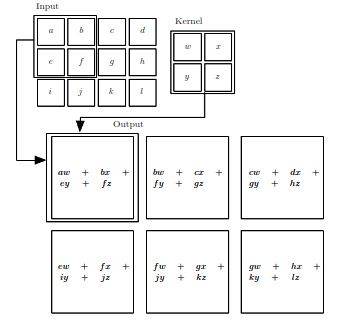
\includegraphics[width=0.45 \textwidth,keepaspectratio=true]{images/convolution.png}
 % convolution.png: 342x321 px, 72dpi, 12.06x11.32 cm, bb=0 0 342 321
 \caption{Abbildung zur Faltung \cite{CNNBook}}
 \label{fig:faltung}
\end{figure}
Mehrere dieser Kernel bilden zusammen ein Teil des Convolutional Layer. Dabei wird der Eingang des Layers wie in Abbildung \ref{fig:cnn} gezeigt auf jeden Kernel mittels der Faltung angewendet. Durch diese Faltung entstehen Erste Feature-Maps. Diese Feature-Maps werden im nächsten Schritt Komponentenweise als Eingabe für eine Aktivierungsfunktion benutzt. In Abbildung \ref{fig:cnn} wird ReLU als Aktivierungsfunktion benutzt\footnote{Für Erklärung Relu siehe \cite{neural}}. Um Overfitting zu vermeiden kann nach dem Anwenden der Aktivierungsfunktion eine Pooling Operation eingeführt werden. Pooling verkleinert die Größe der Feature-Map verkleinert.

Der Begriff Padding aus Abbildung \ref{fig:cnn} enthält einen Wert, der aussagt ob und wenn ja wieviele Pixel um das eigentlich Bild gelegt werden. Dies geschieht, um dem Kernel die Möglichkeit zu geben die Pixel am Rand des Bildes(bzw. der Featuremap der vorherigen Schicht) in mehreren Teilbildern zu verarbeiten.  

Beim Anwenden des Kernels auf die Eingabe kann jedes Teilbild oder weniger Teilbilder verwendet werden. Dies wird über den Parameter Stride kommuniziert. Beim Stride von Eins wird jedes Teilbild verwendet. Wird der Stride auf 2 gesetzt, so wird nach jedem verwendetem Teilbild eines ausgesetzt.


In einem CNN werden mehrere dieser Convolutional Layer hintereinander geschaltet, um komplexe Features erkennen zu können. 
\begin{figure}[H]
  \centering
  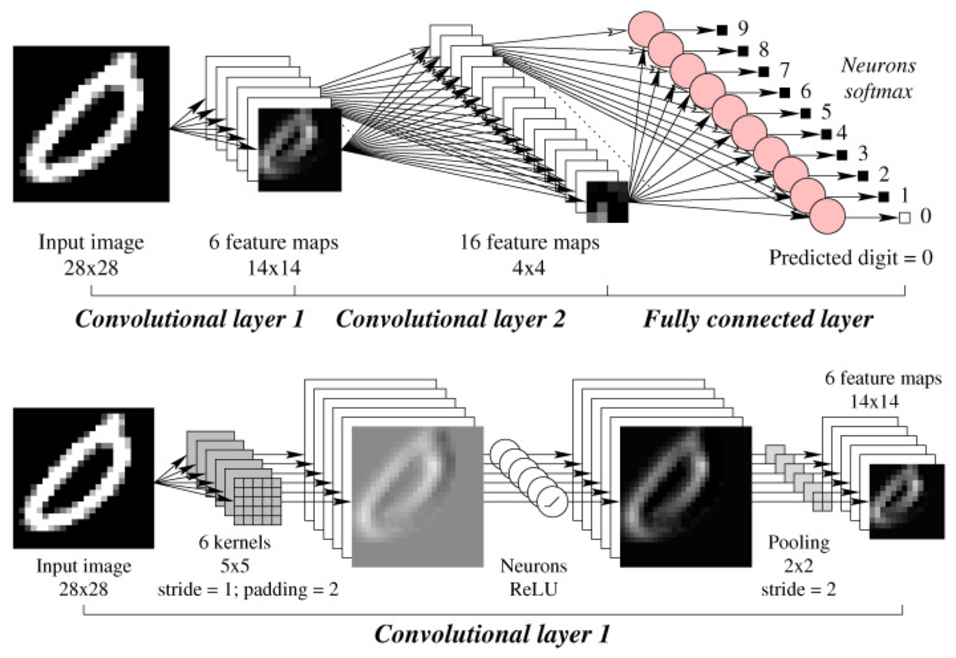
\includegraphics[width=0.75\textwidth]{images/cnn.pdf}
  \caption{Convolutional Neural Net \cite{CNNImg}}
  \label{fig:cnn}
\end{figure}



Eine beispielhafte Übersicht über die CNN-Architektur ist in Abbildung \ref{fig:cnn} zu sehen.

Die Fully-Connected-Layer errechnen aus den Ausgängen der Convolutional-Layer, in welche Klasse ein Objekt klassifiziert werden soll.

Die Filter, die auf die Feature Maps bzw. die Eingabebilder angewendet werden, sind trainierbar. Zusätzlich sind auch die Gewichtungen des Fully-Connected Layers trainierbar. Das heißt durch den Trainingsprozess wird versucht die Werte in der Filtermatrix und des Fully-Connected Layer so zu verändern, dass das gesamte CNN besser klassifizieren kann. 
\color{blue1}

Die Trainingsdaten sind Daten aus dem Datensatz, die bereits klassifiziert sind. Diese Trainingsdaten werden in Batches aufgeteilt. Der Trainingsprozess beginnt mit der Eingabe der Bilder $X_i$ eines Batches von Trainingsdaten hintereinander in die erste Schicht. In jeder Schicht des Netzes wird mit der Eingabe aus der vorherigen Schicht weitergerechnet. In der letzten, voll-verbundenen Schicht ist das Ergebnis eines einzelnen Bildes die Klasse, die durch die aktuellen Belegung der Gewichte des Netzes klassifiziert wird. Aus dieser Klasse und dem vorher vorhandenen Label wird




\color{black}
Für diese Veränderung wird ein Gradientenabstiegsverfahren, welches rückwärts durch die Schichten propagiert wird, benutzt.


\section{ResNet -- eine neuere CNN-Architektur}
Die wachsende Tiefe bei CNN-Architekturen geschieht mit dem Hintergrund, dass tiefere Netze grössere Modellkomplexität haben. Die klassische CNN-Architektur mit hintereinander geschalteten Conv-Layern schafft es bei wachsender Tiefe des Netzes nicht diese Komplexität in bessere Klassifikationsleistung umzusetzen. Die Quelle zu diesem Unterkapitel ist das Paper, welches wegweisend für die Verwendung von Residualen Netzen in der Wissenschaft ist \cite{resnet}.


Neuere CNN-Architekturen schaffen es dieses Problem zu vermeiden. Ein dieser neueren Architekturen ist das ResNet. Das ResNet ist ein Residualnetz, welches Kurzschlussverbindungen einführt. In Abbildung \ref{abb:residual} ist zu sehen wie eine Kurzschlussverbindung aussieht. Durch die Kurzschlussverbindungen in den einzelnen Blöcken ist es für das Netzwerk einfacher Funktionsbestandteile, die ähnlich einer Idenditätsfunktionen sind, zu lernen.   

\begin{figure}[h]
 \centering
 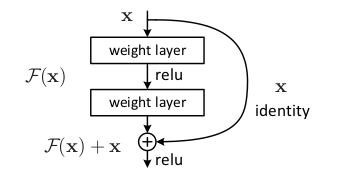
\includegraphics[width=0.5\textwidth]{KapitelPartA/images/kurzschluss.png}
 % kurzschluss.png: 385x188 px, 72dpi, 13.58x6.63 cm, bb=0 0 385 188
 \caption{Abbildung der Kurzschlussverbindung \cite{resnet}}
 \label{abb:residual}
\end{figure}



Vermieden wird damit im Vergleich zu einem klassischen CNN das Problem des verschwindenden Gradientens. Bei einem klassischen CNN wird mit der letzten Schicht begonnen und der Gradient wird durch die Kettenregel bis zur ersten Schicht berechnet. Je Tiefer das Netz wird desto kleiner werden die Veränderungen des Gradienten für die ersten Schichten. Die Gewichte konvergieren dann sehr langsam bzw. teilweise gar nicht mehr in die gewünschten Richtung.


Residuale Netze vermeiden dies, indem sie aus vielen kleineren Netzen bestehen. Hier wird der Gradient nicht auf einer Linie zur Eingangsschicht zurück propagiert, sondern auch über die Kurzschlussverbindungen. So entsteht ein Netz, welches sehr viel tiefer sein kann ohne die Probleme des verschwindenden Gradienten zu haben. Durch das Wegfallen dieses Problems lassen sich mit Residualen Netzen bessere Traningsfehler und Testfehlerraten erreichen.

Eine weitere Technik, die in residualen Netzen verwendet wird ist die der Bottleneck-Blocks. Dies resultiert aus dem Problem der stark steigenden Trainingszeiten je breiter die Blöcke sind. Ein Bottleneck Block ist in Abbildung \ref{abb:bottleneck} abgebildet.

Die erste Schicht im Bottleneck-Block reduziert dabei die Größe der Feature-Map. Dies hat zur Folge, dass die Durchlaufzeit des mittleren Convolutional Layers geringer ist als bei einem Äquivalenten nicht Bottleneck-Block. Das letzte Layer des Blockes stellt die Größe vor dem Block wieder her.

Ein von der Zeitkomplexität ähnlicher Block wie der Block in Abbildung \ref{abb:bottleneck} ist in Abbildung \ref{abb:nonbottleneck} zusehen. Wird in einem 34-Layer residualen Netzwerk aus Blöcken wie in Abbildung \ref{abb:nonbottleneck} jeder Block durch einen Block wie in Abbildung \ref{abb:bottleneck} ausgetauscht, so entsteht ein 50- Layer residual Netzwerk mit einer durchschnittlich erhöhten Accuracy. 


\begin{figure}[h]
 \centering
 \subfloat[][Bottleneck]{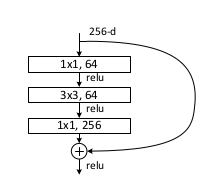
\includegraphics[width=0.4\textwidth]{KapitelPartA/images/bottleneck.png}\label{abb:bottleneck}}
 \qquad
 \subfloat[][Nicht-Bottleneck]{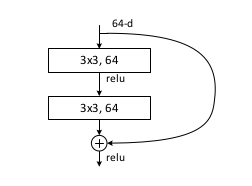
\includegraphics[width=0.4\textwidth]{KapitelPartA/images/plain.png}\label{abb:nonbottleneck}}
       \caption{Vergleich zweier Residual Netz Blöcke \cite{resnet}}
\end{figure}


\section{Vorgehen zur Suche nachdem Stand der Wissenschaft}
Eine Google-Suche nach ``time efficient training convolutional neural networks'' ergibt ungefähr 12 Millionen Suchergebnisse. Mit dieser Flut an Ergebnissen und vielen populär-wissenschaftlichen Einträgen ist die Suche nicht erfolgreich. Aus diesem Grund wird die Suche auf die Seite arvix.org eingeschränkt. Diese Einschränkung macht Sinn mit dem Hintergrund, dass bereits 2017 über 60\% Prozent der publizierten Paper auf arxiv.org als Preprint veröffentlicht wurden \cite{popular}. Diese Zahl ist seitdem weiter gestiegen, was die Zahl der veröffentlichten Paper im Bereich Machine Learning pro Tag in Abbildung \ref{abb:arxiv} zeigt.

\begin{figure}[h]
 \centering
 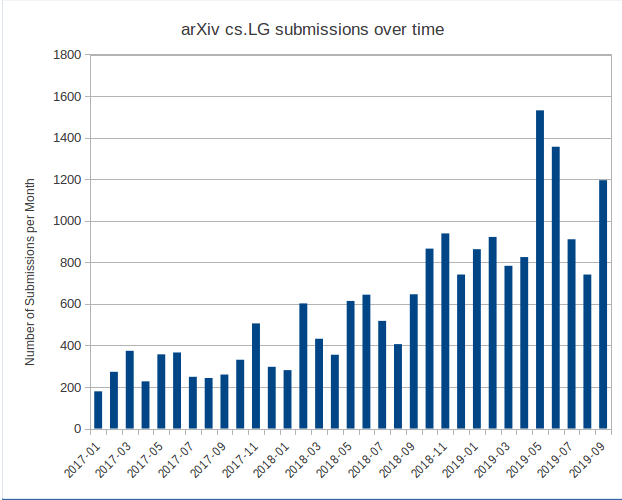
\includegraphics[width=0.5\textwidth]{KapitelPartA/images/arxiv.png}
 % arxiv.png: 622x500 px, 72dpi, 21.94x17.64 cm, bb=0 0 622 500
 \caption{Tägliche Submissionen der Kategory Machine Learning auf arxiv \cite{cornell}}
 \label{abb:arxiv}
\end{figure}


Auch mit der auf arxiv.org eingeschränkten Suche ist die Menge an wissenschaftlichen Veröffentlichungen weiterhin zu groß für eine einzelne wissenschaftliche Arbeit. Zunächst wird eine Vorauswahl anhand des Themas der Arbeit getroffen. Es fallen alle Veröffentlichungen weg, die auf anderen Ausführungsplattformen als GPUs arbeiten. Aufgrund des schnellen Forschungsfortschritts und der Hardware sowie Softwareentwicklung liegt der Fokus auf Veröffentlichungen nach 2016.

Die nach diesen Einschränkungen gefundenen Paper sind in einer Mindmap in Abbildung \ref{abb:mindmap} zu sehen. Mit blauer Schrift werden die Suchbegriffe dargestellt. Die einzelnen aufgrund dieser Suchbegriffe gefundenen Paper werden mit grüner Schrift gezeigt. Mit roter Schrift werden die Paper dargestellt, die durch das Paper der vorherigen Ebene zitiert werden. Gelb hinterlegt sind Paper, die das Paper auf der vorheigen Ebene zitieren. In den weiteren Unterkapiteln werden die so gefundenen Paper vorgestellt und die verwendeten Methoden erklärt. 

\begin{figure}[h]
 \centering
 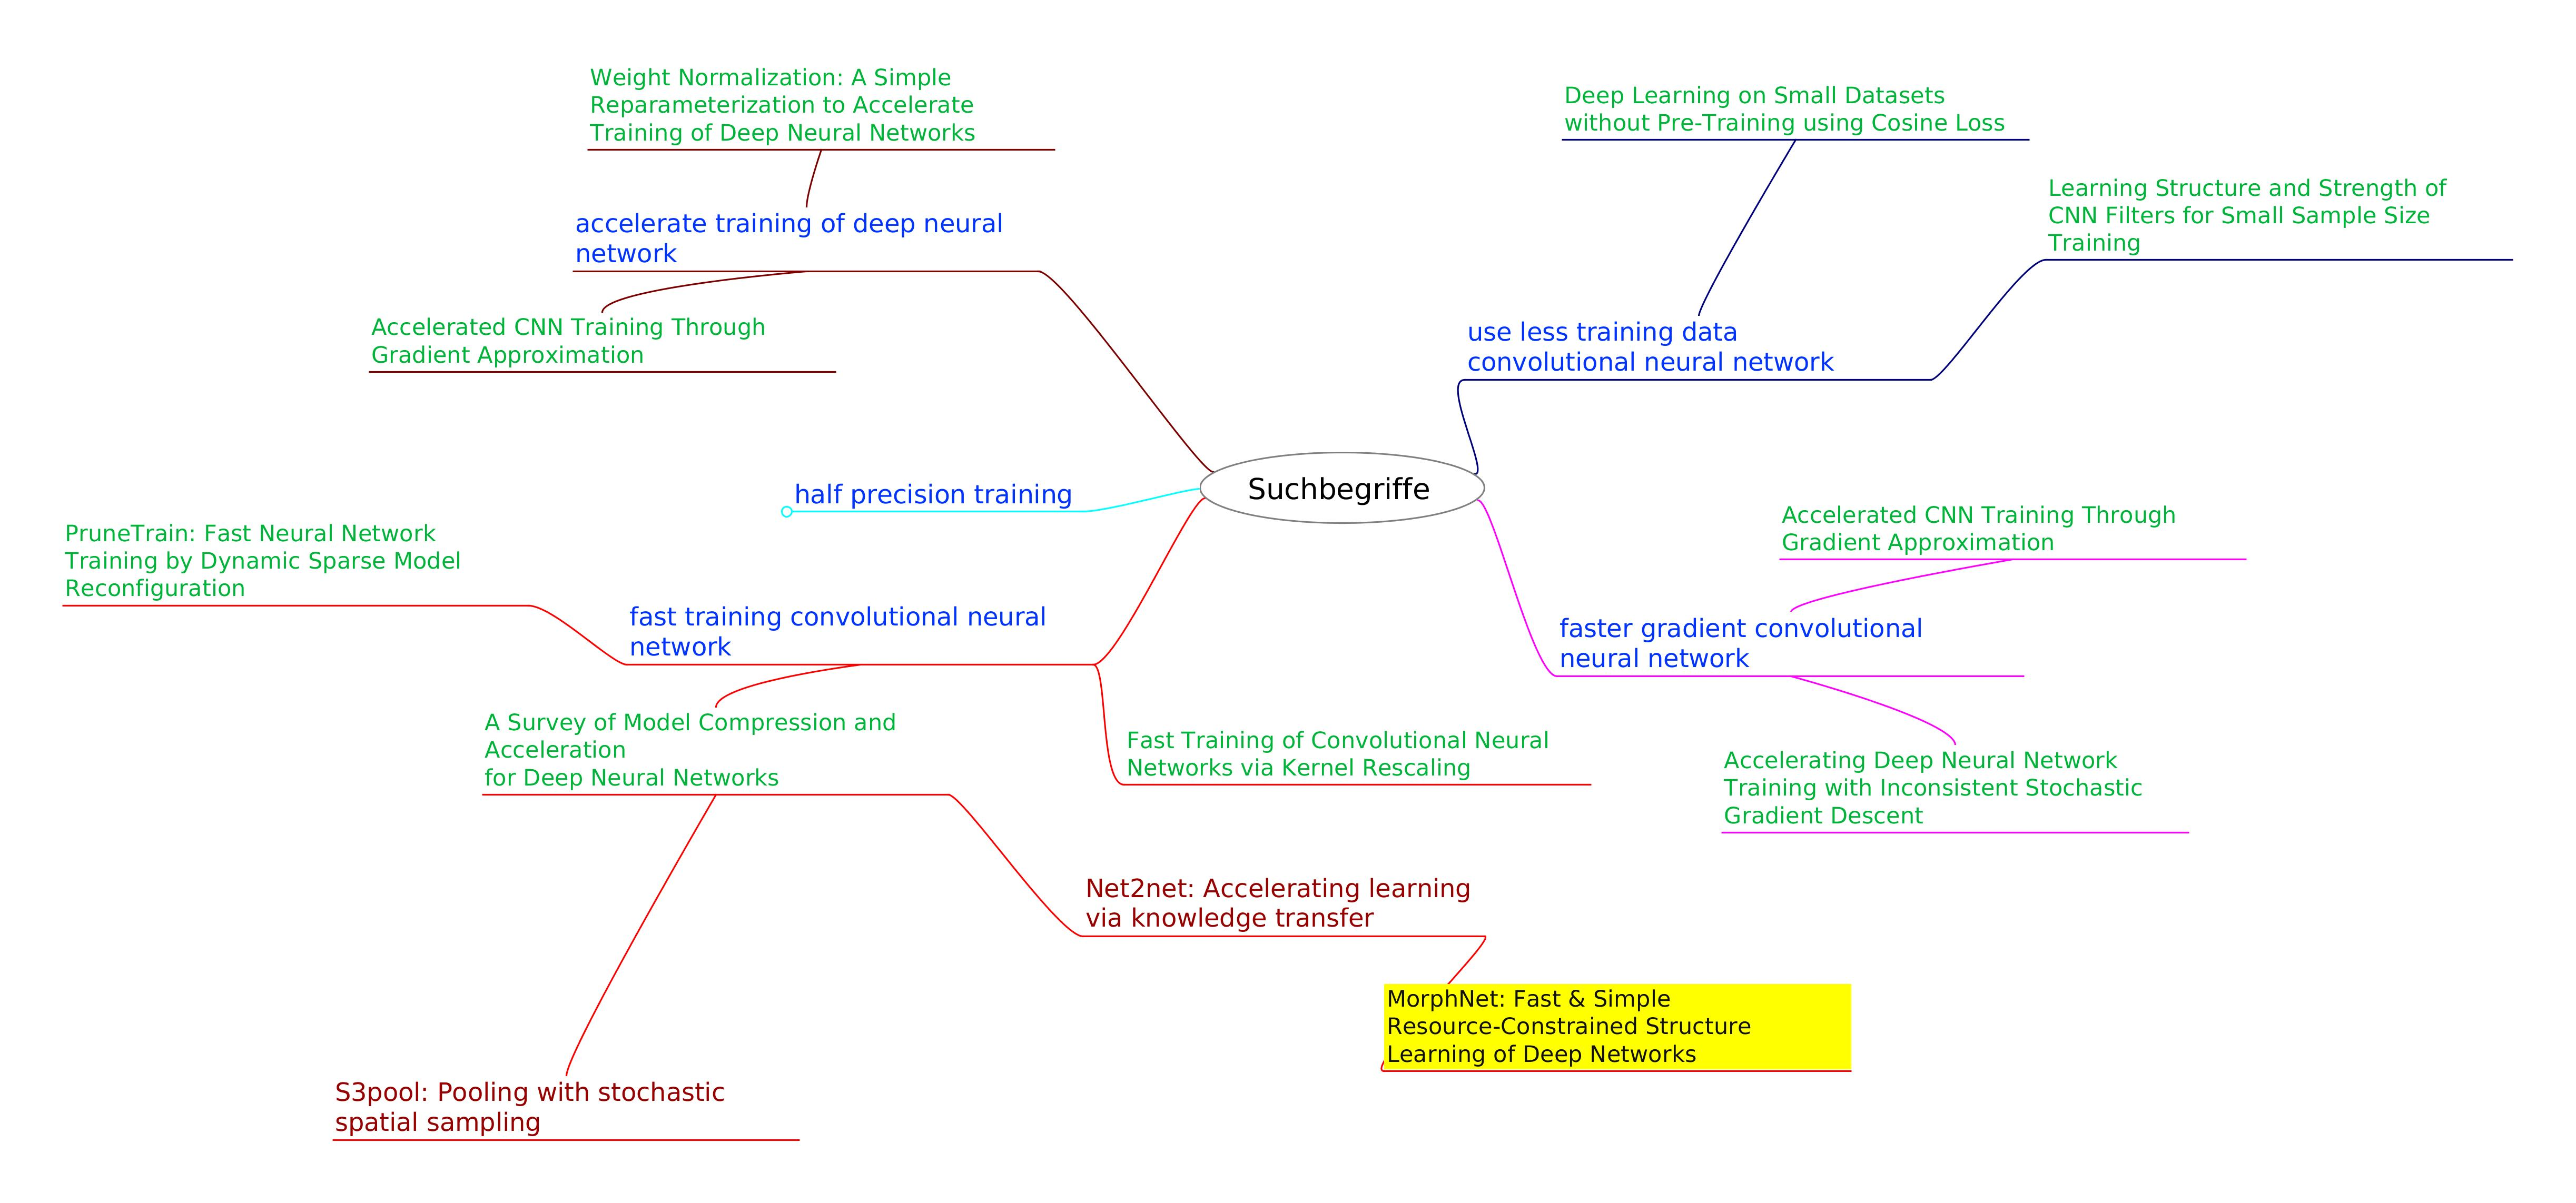
\includegraphics[width=1\textwidth]{KapitelPartA/images/mindmap.jpg}
 % mindmap.jpg: 6907x1207 px, 183dpi, 95.93x16.76 cm, bb=0 0 2719 475
 \caption{Mindmap zu den Suchbegriffen bezüglich des aktuellen wissenschaftlichen Stands}
 \label{abb:mindmap}
\end{figure}


